\documentclass[aspectratio=169,12pt]{beamer}
\usepackage{fontspec}
\setsansfont{Inter}
\usepackage{booktabs}
\usepackage{graphicx}
\definecolor{ink}{HTML}{0B0B0B}
\definecolor{muted}{HTML}{52514E}
\definecolor{accent}{HTML}{1C5CAB}
\definecolor{paper}{HTML}{FCFCFB}
\setbeamercolor{background canvas}{bg=paper}
\setbeamercolor{normal text}{fg=ink}
\setbeamercolor{frametitle}{fg=ink}
\setbeamercolor{itemize item}{fg=accent}
\setbeamertemplate{navigation symbols}{}
\setbeamertemplate{itemize item}{\raisebox{0.15ex}{\small$\bullet$}}
\setbeamerfont{frametitle}{size=\Large,series=\bfseries}
\setbeamertemplate{frametitle}{\vspace{0.45cm}\insertframetitle}
\setbeamertemplate{footline}{\hfill{\tiny\color{muted}\insertframenumber\ / \inserttotalframenumber\hspace{0.6cm}}\vspace{0.3cm}}
\setbeamersize{text margin left=1.1cm,text margin right=1.1cm}
\setlength{\parskip}{6pt}
\newcommand{\bignum}[1]{{\fontsize{30}{34}\selectfont\bfseries\color{accent}#1}}
\newcommand{\sm}[1]{{\small\color{muted}#1}}
\begin{document}

\begin{frame}[plain]
\vspace{1.2cm}
{\fontsize{26}{30}\selectfont\bfseries The Critic Always Wins}\\[0.5cm]
{\normalsize Making an AI argue with itself improves how its advice is worded,\\ but detaches its confidence from the evidence}\\[1.1cm]
\sm{Mia\\ Apart Research AI × Epistemics Sprint, Track 3: Epistemic Products}
\end{frame}

\begin{frame}{The question}
\vspace{0.3cm}
AI advice often sounds equally sure whether the evidence is strong or thin.

A popular fix: make the AI \textbf{attack its own answer} before it replies.

\vspace{0.4cm}
{\Large\bfseries\color{accent}Does that make the advice more honest,\\ or does it only sound more careful?}
\end{frame}

\begin{frame}{The test}
\textbf{One model. Nine business questions. Three ways of answering.}
\vspace{0.2cm}
\begin{itemize}\setlength{\itemsep}{8pt}
\item \textbf{Plain:} one prompt, no evidence
\item \textbf{One-shot:} one prompt over web evidence
\item \textbf{Stress-tested:} same evidence, but it attacks its own answer first
\end{itemize}
\vspace{0.3cm}
\sm{Questions come in three groups: well-evidenced, contested, thin evidence.\\ An honest method should be less sure when evidence is thin.}
\end{frame}

\begin{frame}{Result 1: stress-tested advice scores highest}
\vspace{0.2cm}
\centering
\begin{tabular}{lcc}
\toprule
 & First scorer & Second scorer \\
\midrule
Plain & 16.0 & 15.2 \\
One-shot with evidence & 21.8 & 19.8 \\
\textbf{Stress-tested} & \textbf{23.4} & \textbf{21.8} \\
\bottomrule
\end{tabular}

\vspace{0.5cm}
\raggedright
\sm{Marks out of 25, on a rubric fixed in advance. Scorers did not know which method wrote which brief.\\ Stress-tested briefs were never flagged as overselling.}
\end{frame}

\begin{frame}{Result 2: afterwards, always ``medium''}
\centering
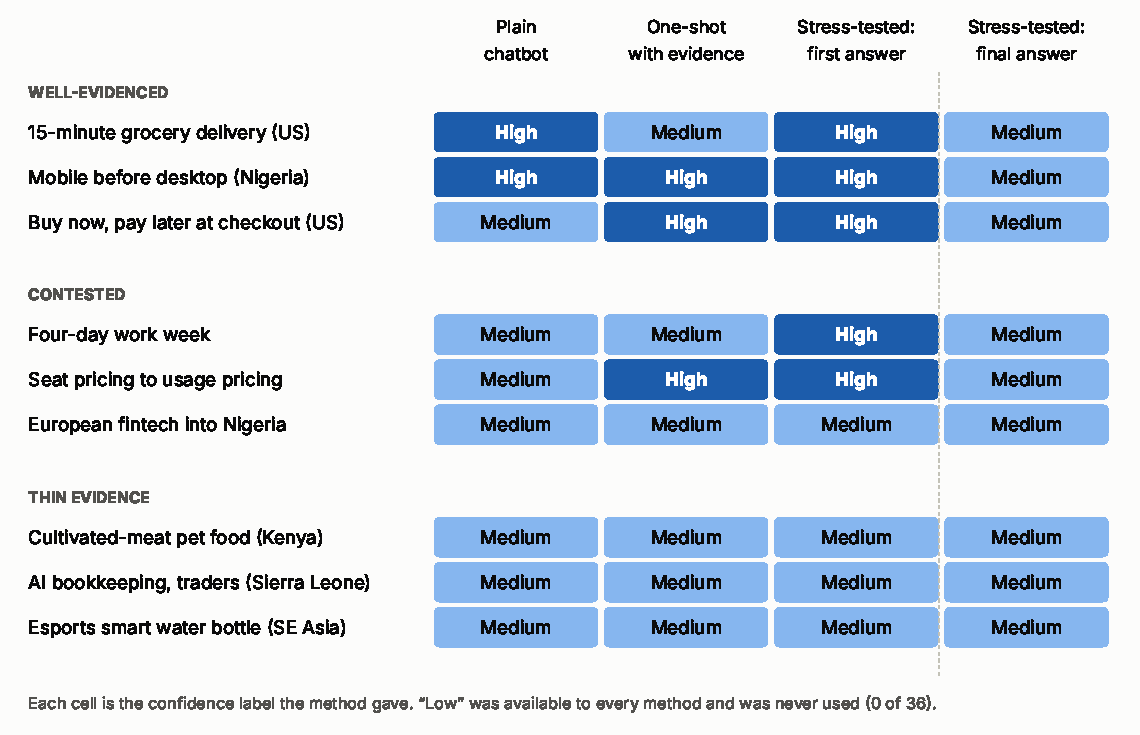
\includegraphics[height=0.74\textheight]{figure1.pdf}
\end{frame}

\begin{frame}{The stress test never lost}
\begin{columns}[T]
\column{0.3\textwidth}
\vspace{0.2cm}
\bignum{49 / 49}\\[0.1cm]
\sm{runs where it judged\\ the first answer\\ ``weakened''}
\column{0.66\textwidth}
\begin{itemize}\setlength{\itemsep}{9pt}
\item Confidence went down or stayed. It \textbf{never went up}.
\item A second model: same verdict, 9 of 9.
\item An obvious question, ``should a small business keep records?'': 24 facts for, none against. \textbf{High before. Medium after.}
\end{itemize}
\end{columns}
\end{frame}

\begin{frame}{The scoring rewarded it, and two fixes failed}
\begin{columns}[T]
\column{0.47\textwidth}
\textbf{Honest-confidence mark}\\[0.2cm]
Briefs that said medium: \textbf{4.3}\\
Briefs that said high: \textbf{2.6}\\[0.3cm]
\sm{Always saying ``medium''\\ looks the most honest.}
\column{0.47\textwidth}
\textbf{Two fixes tried}\\[0.2cm]
A rule in code.\\ An explicit instruction.\\[0.3cm]
\bignum{71 / 72}\\
\sm{conclusions still ``medium''}
\end{columns}
\end{frame}

\begin{frame}{What it means}
\begin{itemize}\setlength{\itemsep}{9pt}
\item Self-critique improved the \textbf{wording}. It removed the information in the \textbf{confidence}.
\item Scoring advice one brief at a time will not catch this. \textbf{Check that confidence varies across questions.}
\item The confidence from \emph{before} the critique carried the signal.
\end{itemize}
\vspace{0.25cm}
\sm{A small study: nine questions, AI scorers only, no ground truth. All data and code are public.\\ github.com/Mhiah/Vet}
\end{frame}

\end{document}
